\section{Intelligent hydraulic manifold used in an injection molding machine}

文献\parencite{US6289259B1}专利所述的是一种用于注塑机的智能液压歧管,该发明解决的是一般电液驱动子系统的诸多不便的问题。

\begin{figure}[!htp]
	\centering
	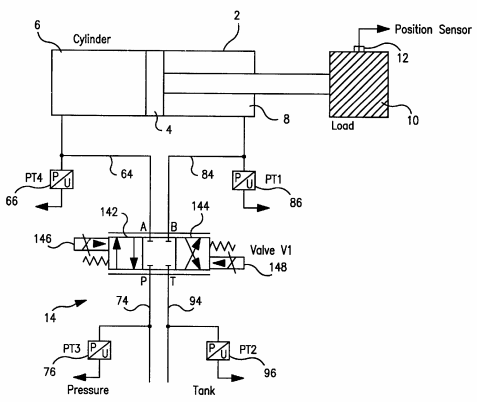
\includegraphics[width=\textwidth]{IMG/drivesubsys.png}
	\bicaption[液压驱动子系统]
		{液压驱动子系统}
		{Hydraulic drive subsystem}
	\label{fig:drivesubsys}
\end{figure}

如图\ref{fig:drivesubsys}是一个带反馈电控换向阀和液压缸组成的驱动系统。这个驱动系统的液压部分并不复杂,三位电磁换向阀接受电压信号工作在某个状态致使液压缸活塞向左、向右或停止运动。

还应该注意到的是,该系统还布置了许多传感器,比如在负载上布置了位置传感器,在管线84、64、74和94的位置布置了液压传感器。布置有传感器的该驱动系统能够构成简单或复杂的闭环控制系统,使得该驱动系统的更加可靠和可控。

布置大量传感器和驱动信号线带来的困扰,是在实际安装、检修过程中涉及数量极多的电子线路。这使得安装检修过程非常困难和低效。另外,这个系统正常工作时会大量占用控制中心的端口等硬件资源和计算资源,在某些高频情况下将给控制中心带来极大地负担。

\begin{figure}[!htp]
	\centering
	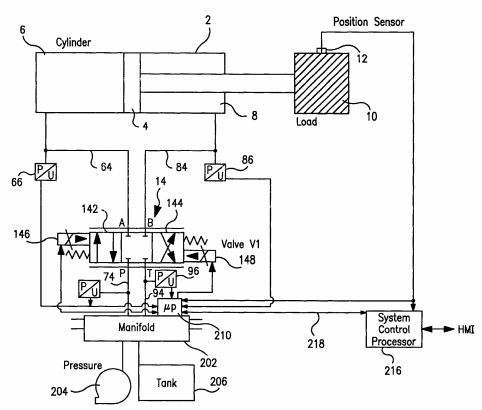
\includegraphics[width=\textwidth]{IMG/manifoldsubsys.png}
	\bicaption[智能液压歧管方案]
		{智能液压歧管方案}
		{Intelligent hydraulic manifold solution}
	\label{fig:manifoldsubsys}
\end{figure}

文献\parencite{US6289259B1}专利提出了一种封装了微控制器的液压歧管的方案。

如图\ref{fig:manifoldsubsys}给出了该发明的应用场景。从图中可以看到,在驱动系统附近的液压歧管202上安装了微处理器210,图中大量的传感器配线不再直接连接到控制中心,而是就近地连接到了微处理器210上。

该解决方案将该驱动部分的控制进行本地化封装,通过将独立的微处理器安装在附近的液压歧管上,并将部分反馈装置直接连接到微处理器上并让微处理器直接控制电控换向阀的控制信号,微处理器可以接收来自系统控制中心的指令,这样极大地解放了系统控制中心的硬件资源和计算资源,同时让安装和检修变得模块化和简单化。

文献\parencite{US6289259B1}专利这个例子体现了电液一体化和模块化液压元件,将控制器嵌入到液压元件中使得该元件有更高的易用用性和可靠性。
